\chapter{Zavedení základních pojmů}
\label{ch:glosary}
Dříve, než se práce začne zabývat problematikou více do hloubky, je třeba si stanovit některé základní pojmy z teorie hudby a stručný popis ukulele. Po více informací bych doporučil odbornou literaturu, např. \cite[Hudební slovník pro každého]{jirivyslouzil_1995_hudebni}.

\section{Základ teorie hudby}
Základ hudby je tón, zvuk s periodickým kmitáním o určité frekvenci, příkladem může být tón \emph{C}. Následně hudební stupnice určuje počet tónů a půltónů a jejich frekvenční vzdálenost. Práce obsahuje pouze stupnice durové a mollové a to v souvislosti s akordy, příkladem může být stupnice \emph{C dur}. Akord je souzvuk několika tónů, u ukulele to je souzvuk čtyř tónů, jeden pro každou strunu. Označení akordů vychází z tónů a vzdálenostmi mezi nimi, které se většinou řídí nějakou stupnicí, např. akord \emph{Emi}, neboli \emph{e moll} se řídí mollovou stupnicí.

\section{Popis ukulele}
\label{sc:ukulele_description}
Ukulele je čtyřstrunný drnkací hudební nástroj, vzhledem podobný malé kytaře. Ukulele původně pochází z~Havajských ostrovů kde vzniklo z~nástroje zvaného Braguinha a o~původu jeho jména se vedou spekulace~\cite{rek_2008_kola}.

Skládá se z dvou hlavních částí - těla a krku. Krk se následně skládá z hmatníku, který tvoří pražce a hlavice s ladící mechanikou. Struny jsou nataženy od kobylky až k ladící mechanice a zpravidla mají různé ladění. Běžné ladění udává ladění jednotlivých strun od shora dolů.

\subsection{Hra na ukulele}
Samotné hraní je velmi podobné hře na kytaru –⁠ ukazováček, prostředníček, prsteníček a malíček levé ruky přitiskávají struny mezi pražci, čímž určují akord a prsty pravé ruky přejíždějí po strunách někde na pomezí krku a těla ukulele. Způsobů, jak držet akordy, je několik a většinou záleží na dalším, resp. předchozím akordu, aby si hráč zjednodušil přechod. Stejně tak je i více způsobů jak přejíždět prsty po strunách. Prsty mohou jet dolů, nebo nahoru a to břískem nebo nehtem prstu, či lehce klepnout do těla a tím zároveň utlumit struny. Různým kombinacím těchto pohybů se říká strumming pattern.

\subsection{Typy ukulele}
Ukulele má několik variant, které se odlišují velikostí nástroje a barvou zvuku. Nejběžnější a zároveň doporučované pro začátečníky je ukulele sopránové. Sopránové ukulele je zároveň nejmenší a jeho běžné ladění je \textit{g,c,e,a} nebo \textit{a,d,f\textsuperscript{\#},h}.

Další ukulele jsou koncertní a tenorové, které jsou větší, ale ladí se stejně jako ukulele sopránové. Rozdíl je tedy v~barvě zvuku a velikosti, tedy pohodlnosti držení.

Největší ukulele je barytonové, které je běžně laděné stejně jako vrchní čtyři struny kytary, tedy \textit{d,g,h,e}, a je vhodné pro hráče kteří již umí hrát na kytaru, právě kvůli stejnému ladění.

Další, méně obvyklé, verze ukulele jsou šestistrunné, osmistrunné, desetistrunné a uke-bendžo (bendžolele), které vzniklo spojením ukulele a benža.

\begin{figure}
    \centering
    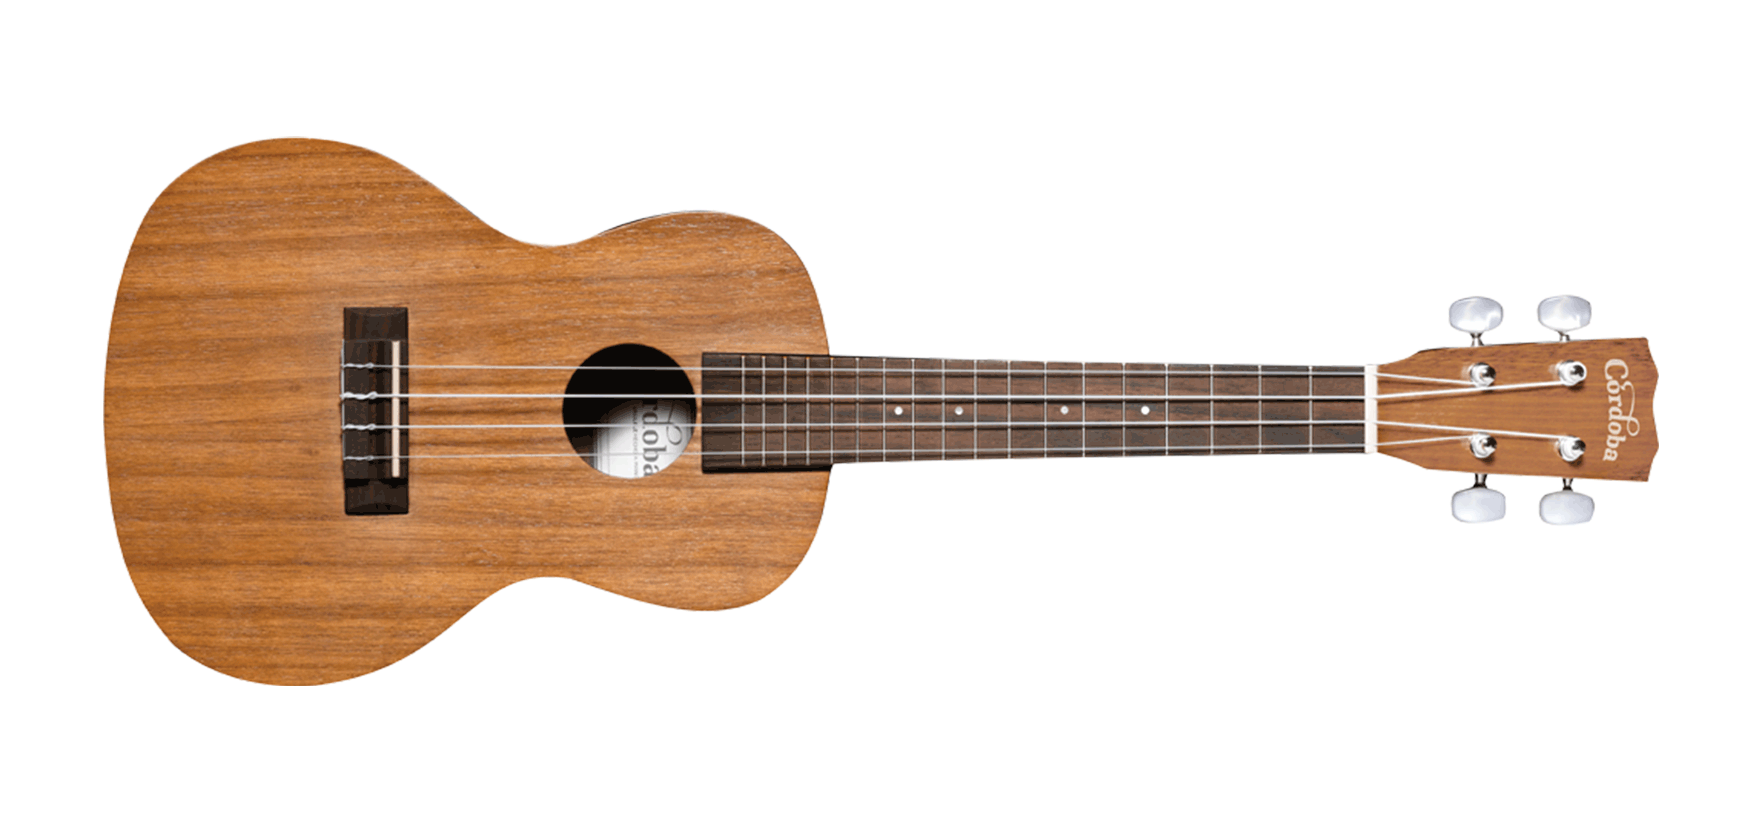
\includegraphics[width=\textwidth]{assets/ukulele.png}
    \caption[Příklad koncertního ukulele]{Příklad koncertního ukulele \cite{cordobaguitars_2020_ukulele}}
    \label{fig:class_diagram}
\end{figure}